%%%
% Author: Yihong Liu (https://liu-yihong.github.io/)
% Repository:
% License: GNU GPL v3.0
% This repository contains an unofficial LaTex beamer
% template for the University of Texas at Dallas.
% Copyright (c) 2022 Yihong Liu
%%%
\documentclass[
	xcolor={svgnames},
	hyperref={pagebackref,bookmarks},
	% aspectratio=169,
	aspectratio=43,
]{beamer}

\mode<presentation>
%%%
% Author: Yihong Liu (https://liu-yihong.github.io/)
% Repository:
% License: GNU GPL v3.0
% This repository contains an unofficial LaTex beamer template for the University of Texas at Dallas.
% Copyright (c) 2022 Yihong Liu
%%%
\usepackage[utf8]{inputenc}
\usepackage{xcolor}
\usepackage{tikz}
% \usepackage{fontawesome5}
\usepackage{fontawesome}
%%%
% Author: Yihong Liu (https://liu-yihong.github.io/)
% Repository:
% License: GNU GPL v3.0
% This repository contains an unofficial LaTex beamer template for the University of Texas at Dallas.
% Copyright (c) 2022 Yihong Liu
%%%
\usetheme{AnnArbor} % Dresden Berlin Madrid Singapore Frankfurt Montpellier
\usecolortheme{crane}
% https://www.cpt.univ-mrs.fr/~masson/latex/Beamer-appearance-cheat-sheet.pdf
\definecolor{utdorange}{RGB}{232,117,0}
\definecolor{utdgreen}{RGB}{18,71,52}
\definecolor{utdcyan}{RGB}{95,244,183}
\definecolor{utdcyangray}{RGB}{138,141,143}

\setbeamercolor*{structure}{bg=utdorange!40,fg=utdorange}

\setbeamercolor*{palette primary}{use=structure,fg=white,bg=structure.fg}
\setbeamercolor*{palette secondary}{use=structure,fg=white,bg=structure.fg!75}
\setbeamercolor*{palette tertiary}{use=structure,fg=white,bg=utdgreen}
\setbeamercolor*{palette quaternary}{fg=white,bg=structure.fg}

\setbeamercolor*{palette sidebar primary}{use=structure,fg=white,bg=structure.fg}
\setbeamercolor*{palette sidebar secondary}{use=structure,fg=white,bg=structure.fg!75}
\setbeamercolor*{palette sidebar tertiary}{use=structure,fg=white,bg=utdgreen}
\setbeamercolor*{palette sidebar quaternary}{fg=white,bg=structure.fg}

\setbeamercolor*{section in toc}{fg=black,bg=white}
% \setbeamercolor{alerted text}{use=structure,fg=utdcyan}
\setbeamercolor{block title alerted}{use=structure,bg=utdcyan}

\setbeamercolor{titlelike}{parent=palette primary,fg=white,bg=utdorange}
\setbeamercolor{frametitle}{bg=utdorange!85,fg=white}
% \setbeamercolor*{titlelike}{parent=palette primary}
%%%
% Author: Yihong Liu (https://liu-yihong.github.io/)
% Repository:
% License: GNU GPL v3.0
% This repository contains an unofficial LaTex beamer template for the University of Texas at Dallas.
% Copyright (c) 2022 Yihong Liu
%%%
% https://tex.stackexchange.com/questions/443659/how-to-remove-date-from-footnote-of-madrid-theme-of-beamer-and-use-that-space-fo
\makeatletter
\setbeamertemplate{footline}{%
  \leavevmode%
  \hbox{%
    \begin{beamercolorbox}[wd=.15\paperwidth,ht=2.25ex,dp=1ex,center]{author in head/foot}{CS5150}%
%      \usebeamerfont{author in head/foot}\insertshortauthor\expandafter\ifblank\expandafter{\beamer@shortinstitute}{}{~~\insertshortinstitute}
    \end{beamercolorbox}%
    \begin{beamercolorbox}[wd=.77\paperwidth,ht=2.25ex,dp=1ex,center]{title in head/foot}%
      \usebeamerfont{title in head/foot}\insertshorttitle
    \end{beamercolorbox}%
  }%
  \begin{beamercolorbox}[wd=.08\paperwidth,ht=2.25ex,dp=1ex,right]{date in head/foot}%
    \usebeamerfont{date in head/foot}%
    \usebeamertemplate{page number in head/foot}%
    \hspace*{2ex}
  \end{beamercolorbox}
  \vskip0pt%
}
\makeatother
%gets rid of bottom navigation symbols
\setbeamertemplate{navigation symbols}{}
%gets rid of bottom navigation bars
% \setbeamertemplate{footline}[frame number]{}
%gets rid of footer
% \setbeamertemplate{footline}{}
%%%
% Author: Yihong Liu (https://liu-yihong.github.io/)
% Repository:
% License: GNU GPL v3.0
% This repository contains an unofficial LaTex beamer template for the University of Texas at Dallas.
% Copyright (c) 2022 Yihong Liu
%%%
\newcommand{\presentationtitle}{}
\newcommand{\presentationsubtitle}{}
\newcommand{\presenter}{}
\newcommand{\department}{}
\newcommand{\school}{}
\newcommand{\university}{}
\newcommand{\email}{}
\renewcommand{\presentationtitle}{Anonymous Authentication with Revocation and Encryption Scheme for V2X}
\renewcommand{\presenter}{Taha Adeel Mohammed}
\renewcommand{\department}{Computer Science and Engineering}
\renewcommand{\school}{IITH}
\renewcommand{\university}{Indian Institute of Technology Hyderabad}
\renewcommand{\email}{\href{mailto:cs20btech11052@iith.ac.in}}
%%%
% Author: Yihong Liu (https://liu-yihong.github.io/)
% Repository:
% License: GNU GPL v3.0
% This repository contains an unofficial LaTex beamer template for the University of Texas at Dallas.
% Copyright (c) 2022 Yihong Liu
%%%
\hypersetup{
    pdfauthor={\presenter},%
    pdftitle={\presentationtitle - \presentationsubtitle},%
    pdfsubject={\department},%
    pdfkeywords={\department, \school, \university},%
    pdfproducer={LaTeX},%
    pdfcreator={pdfLaTeX},
    % bookmarks,
    bookmarksnumbered = true,
    bookmarksopen     = true,
    % pdfpagelabels     = true,
    pdfstartview={XYZ null null 1.2}
}

%% End of Template

\usepackage{blkarray}
\usepackage{amsmath}
\usepackage{amsfonts}
\usepackage{amssymb}
\usepackage{mathtools}

\title[]{Anonymous Authentication with Revocation and Encryption Scheme for V2X}

\title{\presentationtitle}
\author{\presenter}
\institute[IITH]{
	\university\\
}
\date{\today}

\makeatletter
\makeatother

\begin{document}

\AtBeginSection[]{
	\begin{frame}
		\vfill
		\centering
		\begin{beamercolorbox}[sep=8pt,center,shadow=true,rounded=true]{title}
		\usebeamerfont{title}\insertsectionhead\par%
		\end{beamercolorbox}
		\vfill
	\end{frame}
}

\newcommand{\brak}[1]{\ensuremath{\left( #1 \right)}}
\newcommand{\sbrak}[1]{\ensuremath{\left[ #1 \right]}}
\newcommand{\Exp}[1]{\ensuremath{\mathbb{E} \left[ #1 \right]}}
\newcommand{\Var}[1]{\ensuremath{\text{Var} \left[ #1 \right]}}
\setbeamercolor{alerted text}{fg=orange}

\begin{frame}
	\titlepage
\end{frame}


\begin{frame}{Reference}
	\begin{block}{Title}
		PEREA: Towards Practical TTP-Free Revocation in Anonymous Authentication
	\end{block}
	\begin{block}{Authors}
		\begin{itemize}
			\item Patrick P. Tsang - Department of CS, Dartmouth College, USA
			\item Man Ho Au - University of Wollongong, Australia
			\item Apu Kapadia - Department of CS, Dartmouth College, USA
			\item Sean W. Smith - Department of CS, Dartmouth College, USA
		\end{itemize}
	\end{block}
	\begin{block}{Year of Publication}
		\begin{itemize}
			\item 2008
		\end{itemize}
	\end{block}
\end{frame}

\begin{frame}{Contents}
	\tableofcontents
\end{frame}

\section{Additional Design Goals}
\begin{frame}{Additonal Design Goals}
	\begin{block}{Revocation}
		\begin{itemize}
			\item Users should be able to revoke their credentials if they wish to do so, hence allowing for self-revocation.
			\item The Road Side Units (RSUs)/Issuing Authority (IA) should be able to revoke the credentials of a user in a privacy preserving manner if it suspects that the user is malicious.
			\item The revocation should work with our randomized credentials and users should remain unlinkable accross multiple authentications.
		\end{itemize}
	\end{block}
\end{frame}

\section{High Level Overview}
\begin{frame}{High Level Overview}
	\begin{itemize}
		\item Similarly to our original scheme, the user has secrets $\alpha, \beta \in \mathbb{Z}_q^*$, which it uses to register with the IA, getting credentials $(a, b, c, d)$.
		\item These credentials can be used for authentication and deriving the secret key for encrypted CAMs during authentication.
		\item<alert@+> Additionally, to support revocation of misbehaving users, we have each user also present a fresh ticket $t_k$ to the RSU during authentication, and maintain a queue of the past $K$ tickets it used for authentication.
		\item<alert@+> And we have the RSU maintain a blacklist of tickets belonging to misbehaving users.
	\end{itemize} 
\end{frame}

\begin{frame}{High Level Overview}
	\begin{itemize}
		\item<alert@+> During authentication, we have the user prove in zero-knowledge that the last $K$ tickets in its queue haven't been blacklisted by the IA.
		\item<alert@+> We also have the user prove in zero knowledge that the queue of last $K$ tickets is correctly formed.
		\item<alert@+> After verifying the user's credentials, the integrity of the queue, and that the user hasnt been blacklisted, the RSU computes a witness for the ticket $t_k$ and a signature on the queue and shares it with the user.
		\item<alert@+> The user can then use this signature and witness during its next authentication to prove to the RSU in zero-knowledge of the validity of his credentials.
	\end{itemize}
\end{frame}

\begin{frame}{High Level Overview}
	% Insert a centered image in this frame
	\centering
	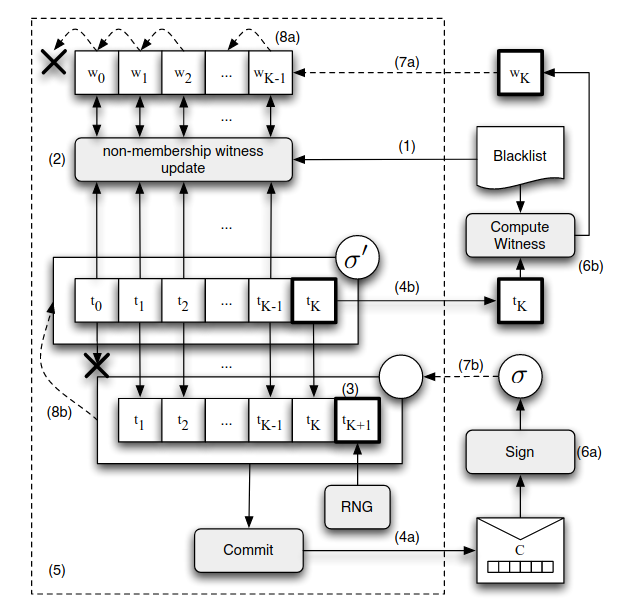
\includegraphics[width=0.6\textwidth]{images/modified-scheme.png}
\end{frame}
			

\section{Building Blocks}

\subsection{Preliminaries}
\begin{frame}{Preliminaries}
	\begin{block}{Bilinear Pairings}
		Let $G$ and $G_T$ be groups of prime order $q$. A map $e : G \times G \rightarrow G_T$ must satisfy the following properties:
		\begin{itemize}
			\item \textit{Bilinearity}: a map $e : G \times G \rightarrow G_T$ is bilinear if $e(a^x, b^y)t = e(a, b)^{xy}$;
			\item \textit{Non-degeneracy:} for all generators $g, h \in G, e(g, h)$ generates $G_T$ ;
			\item Efficiency: There exists an efficient algorithm $BMGen(1^k)$ that outputs $(q, G, GT , e, g)$ to generate the bilinear map and an efficient algorithm to compute $e(a, b)$ for any $a, b \in G$.
		\end{itemize}
	\end{block}
\end{frame}

\subsection*{Hardness Assumptions}
\begin{frame}{Hardness Assumptions}
	The security of our scheme depends on the following number-theoretic hardness assumptions:
	\begin{block}{Strong RSA Assumption}
		The Strong RSA Assumption says that there exists no PPT algorithm which, on input $N$ and $u \in \mathbb{Z}_N^* $ , returns $e > 1$ and $v$ such that $v^ e = u \mod N$, with non-negligible probability (in $\lambda$).
	\end{block}
	\begin{block}{DDH Assumption}
		The Decisional Diffie-Hellman (DDH) Assumption says that there exists no PPT algorithm which, on input quadruple $(g, g^a, g^b, g^c) \in QR_N^4,$, where $a, b \in_R \mathbb{Z}_{|QR_N |}$, and $c \in_R Z_{|QR_N|}$ or $c = ab$ with equal probability, correctly distinguishes which is the case with probability non-negligibly (in $\lambda$) greater than $1/2$.
	\end{block}
\end{frame}

\subsection*{Zero Knowledge Proof of Knowledge Protocols}
\begin{frame}{ZKPoK Protocols}
	\begin{itemize}
		\item A \textit{Zero-Knowledge Proof-of-Knowledge (ZKPoK)} protocol is a protocol in which a prover convinces a verifier that some statement is true without the verifier learning anything except the truth of the statement.
		\item Eg: $PK \{(x) : y = g^x\}$ denotes a
		ZKPoK protocol that proves the knowledge of an integer $x$ such that $y = g^x$ holds, where the value $x$ is secret to the prover.
	\end{itemize}
\end{frame}

\subsection{Tickets and Queues}
\begin{frame}{Tickets and Queues}
	\begin{itemize}[<alert@+>]
		\item The user picks a ticket uniformally at random from the set of primes of atmost $l_t$ bits, where $l_t$ is 166. 
		\item As there are atleast $2^{160}$ tickets, the probability of two randomly chosen tickets colliding is atmost $2^{-80}$.
		\item We represent the queue maintained by the user as
		\vspace*{-3mm} $$Q = \{t_0, t_1, \dots, t_{k-1}\}$$
	\end{itemize}
\end{frame}

\subsection{Accumulator Scheme for Tickets}
\begin{frame}{Accumulator Scheme for Tickets}
	\begin{itemize}[<alert@+>]
		\item We require that the users should be able to successfully prove that they have not been blacklisted by the IA, without revealing their tickets.
		\item Hence for this, we make use of Universal Dynamic Accumulators (UDAs), introduced by Li et al, which allows for an efficient ZKPoK of non-membership in time independant of number of accumulated values.
	\end{itemize}
\end{frame}
\begin{frame}{Accumulator Scheme for Tickets}
	The accumulator has a value V when values $S_T = \{ t_0, t_1, \dots, t_T \} $ are accumulated in it. We can perform the following operations with the help of the accumalator: 
	\begin{itemize}[<alert@+>]
		\item  $Accumulate(V, t_k)$ which outputs the updated value of the accumulator $V'$ that now also contains $t_k$.
		\item Each ticket $t$ not in $S_T$ has a corresponding non-membership witness $w$, such that $IsNonMember(t, V, w) = 1$ holds.
		\item This $w$ can be computed using knowledge of the secret key of the accumulator using $ComputeWitness(t, V, sk_{acc})$.
		\item Given (t, w) for an accumalator value V, anyone can update the witness w to a new witness w' for the updated accumulator value V' using $UpdateWitness(w, t, V, V')$.
	\end{itemize}
\end{frame}

\subsection{Protocol for Queue Signing}
\begin{frame}{Protocol for Queue Signing}
	\begin{itemize}[<alert@+>]
		\item The RSU needs to verify the integrity of the queue, since otherwise a user could circumvent revocation by fabricating a queue with an incorrect set of K tickets.
		\item For this, normal digital signatures are not sufficient, as they will immediately allow the RSU to link the user to past actions. 
		\item We require the verification to happen without revealing either the queue or the signature on it.  
		\item For this, we utilize the signature scheme given by Camenisch and Lysyanskaya for a block of messages, adapted for our scheme.
	\end{itemize}
\end{frame}

\begin{frame}{Protocol for Queue Signing}
	This signature scheme allows us to perform the following necessary operations and ZKPoKs: 
	\begin{itemize}[<alert@+>]
		\item \textbf{Proof of knowledge of a signed queue: } This protocol allows a user to prove to the RSU the possession of a valid signature without revealing the queue and signatures themselves. 
		\item \textbf{Proof of relation between two queues: }
		\begin{itemize}
			\item During authentication, the user updates his queue from $Q$ to $Q' = Q.Enq(t_k).Deq()$ for use during the next authentication.
			\item This proof allows the user to convince to the RSU that $Q'$ was indeed correctly updated from $Q$.
		\end{itemize}
	\end{itemize}
\end{frame}

\section{Modified Scheme Construction}
\begin{frame}{Modified Scheme Construction}
	Using the above mentioned building blocks, we can construct a modified scheme as follows:
	\begin{block}{Setup}
		\begin{itemize}
			\item For the randomizable signatures using bilinear pairings, the IA chooses a Type-3 pairing with the parameters $(e, g_1, g_2, g, G_1, G_2, G)$, and $(sk, pk) = ((x, y), (X=g_2^x, Y=g_1^y))$, where $x, y \in \mathbb{Z}_q^*$
			\item Depending on the system requirements, the IA decides on an appropriate revokation window size $K$. For our scheme, small values of $K$, such as $K=10$, would also be sufficient.
			\item The IA also initializes the accumalator, blacklist, and the parameters of the signature scheme for the queue.
		\end{itemize}
	\end{block}
\end{frame}

\begin{frame}{Modified Scheme Construction}
	\begin{block}{Registration}
		\begin{itemize}
			\item The user has secrets $(\alpha, \beta) \in_R \mathbb{Z}_q^*$, and sends $req = (a = g_1^{\beta}, b = a^{\alpha})$ to the IA. The IA verifies the user and outputs the signature $\sigma = (a, b, c = a^x, d = (bc)^y)$ to the user.
			\item Also the user picks a random ticket $t$ and initializes his queue as $ Q = \{ \hat{t}, \hat{t}, \dots, \hat{t}, t \} $, where $\hat{t}$ is a dummy ticket provided by the IA.
			\item Then the user engages in the ZKPoKs to prove his queue is well formed, and to get the witness for the ticket and signature for the queue.
			\item Finally, the user stores his credentials as \vspace*{-2mm}
			$$ cred = (\sigma, t, Q, (w_i)_{i=0}^{K-1}, \sigma', BL, V) $$
		\end{itemize}
	\end{block}
\end{frame}

\begin{frame}{Modified Scheme Construction}
	\vspace*{-2mm}
	\begin{block}{Authentication}
		\begin{itemize}
			\item \textbf{Randomizable Signature check: } The user shares $\sigma^r = (a^r, b^r, c^r, d^r)$, which the RSU verifies by checking that $e(a^r, X) = e(c^r, g_2)$ and $e(d^r, g_2) = e(bc^r, Y)$.
			\item \textbf{Blacklist Check: } The user obtains the current blacklist from the RSU, and verifies that he hasn't been revoked.
			\item \textbf{Request for authentication: } 
			\begin{itemize}
				\item Using the updated value of the blacklist, the user updates the witness for each ticket in his queue, and generates a fresh ticket $t^*$.
				\item Then he engages with the RSU in the ZKPoKs to prove that his queue is well formed, and that none of his tickets have been revoked.
			\end{itemize}
			\item \textbf{Refreshment issuing: } After verifying the user, the RSU computes the witness and signature for the queue, and sends it to the user.
			\item \textbf{Credential Refreshment: } Finally the user updates his credentials for the next authentication using the signature and witness.
		\end{itemize}
	\end{block}
\end{frame}

\begin{frame}{Modified Scheme Construction}
	\begin{block}{Revocation}
		\begin{itemize}
			\item To blacklist a misbehaving user who provided $t_k$, the RSU/IA updates the blacklist as $BL' = BL \cup \{ t_k \}$, and updates the accumulator as $V' = Accumulate(V, t_k)$.
			\item The next time the misbehaving user tries to authenticate, he will be unable to prove that $t_k$ from his queue is not in the accumulator. Hence he won't be authenticated.
		\end{itemize}
	\end{block}
	\begin{block}{Key generation and Encryption Scheme}
		After the authentication in the above steps, the rest of the construction for key generation and sharing of encrypted CAMs can be done similarly to the original scheme.
	\end{block}
\end{frame}

\section{Limitations}
\begin{frame}{Limitations}
	\begin{itemize}
		\item While the above proposed scheme allows us to have privacy enhanced revocation in V2X, it significantly impacts the efficiency of the scheme.
		\item For each authentication, the user now has to perform the ZKPoKs for each value in the queue. This significantly increases the computation and communication overheads, which is not very acceptable for V2X applications.
	\end{itemize}
\end{frame}

\begin{frame}
	\begin{center}
		\huge Thank you!
	\end{center}
\end{frame}

\end{document}